\refstepcounter{section}
\section*{Lecture 30: Lie Derivatives}
\addcontentsline{toc}{section}{Lecture 30: Lie Derivatives}
We will shift our focus from the physical aspects to a more mathematical aspect, of finding the symmetries of a given arbitrary metric. Coordinate transformations which keep the metric invariant are called \textit{isometries}\footnote{Mathematically,  \textit{isometries} are \textit{diffeomorphisms} such that the \textit{pullback} of the metric is equal to the metric, which basically means that isometries preserve the metric, but this is justsome sophisticated differential geometric jargon, made up to sound cool (and also to precisely define things without being philosophical and hand-wavy)}. Recall the transformation of different tensorial quanttities, where now, the dependence on the coordinates is explicitly shown:
\begin{itemize}[label=$\blacktriangleright$]
    \item \textbf{Scalar}: $\varphi'(x') = \varphi(x) $
    \item \textbf{Vector}: $v^{\mu '}(x') = \trmat{\mu}{\nu} v^{\nu}(x)$
    \item \textbf{(0,2) Tensor}: $L_{\mu\nu}'(x') = \itrmat{\beta}{\nu}\itrmat{\alpha}{\mu}L_{\alpha\beta}(x)$
\end{itemize}
We need a general procedure to find the isometries of a given metric. For that, let us now consider an infinitesimal coordinate transformation by some vector $\xi^\mu$
$$x'^\mu = x^\mu + \varepsilon \xi^\mu(\fvec{x})\qquad 0<\varepsilon\ll 1\ $$
The transformation matrix, upto order $\SO(\varepsilon^2)$, for the above transformation is given as:
\begin{align*}
    \trmat{\mu}{\nu} = \pdv{x'^\mu}{x^\nu} = \pdv{x^\nu}\qty(x^\mu + \varepsilon \xi^\mu) = \tensor{\delta}{^\mu _\nu}+\varepsilon\pdv{\xi^\mu}{x^\nu}
\end{align*}
The inverse transformation is similarly given as:
$$ \itrmat{\mu}{\nu} =\tensor{\delta}{^\mu _\nu}-\varepsilon\pdv{\xi^\mu}{x^\nu}$$
We can check that this is indeed the inverse upto $\SO(\varepsilon^2)$, since 
\begin{align*}
    \trmat{\alpha}{\nu}\itrmat{\nu}{\beta} &= \qty( \tensor{\delta}{^\alpha _\nu}+\varepsilon\pdv{\xi^\alpha}{x^\nu})\qty(\tensor{\delta}{^\nu _\beta}-\varepsilon\pdv{\xi^\nu}{x^\beta})\\
    &=\tensor{\delta}{^\alpha _\beta} + \varepsilon\qty[\pdv{\xi^\alpha}{x^\nu} \tensor{\delta}{^\nu _\beta}-\pdv{\xi^\nu}{x^\beta} \tensor{\delta}{^\alpha _\nu}]\\
    &=\tensor{\delta}{^\alpha _\beta} + \varepsilon\qty[\cancel{\pdv{\xi^\alpha}{x^\beta}}-\cancel{\pdv{\xi^\alpha}{x^\beta}} ]\\
    &=\tensor{\delta}{^\alpha _\beta}
\end{align*}
NOTE: In the following part, we will define a new kind of derivative called the \textit{Lie derivative}. We will use the notion of coordinate transformations to define this, however, the precise definition is by considering the `flow' generated by some vector field.\\[0.2cm]
There is a nice reason for such a definition of the Lie derivative. Suppose $\boldsymbol{\xi}$ is a vector field, which means that, if we specify a point in spacetime, $\boldsymbol{\xi}$ will assign a vector to that point. Now we can define some curves (called \textit{flow lines} or \textit{integral curves}) such that at each point $p$ on the curve, if we define a tangent vector, this tangent vector will be equal to the vector that is assigned by $\boldsymbol{\xi}$ at $p$. \\[0.2cm] 
Consider a flow-line curve parameterised by some $\varepsilon$, $\upsigma(\varepsilon)$ generated by the vector field $\boldsymbol{\xi}$ and a point $p$ with coordinates $x^\mu$ on that flow-line. We want to compare how some given vector field, say $T$, changes when we move along the flow line to point $q$.\\[0.2cm] At each point on the flow line, $T$ will have different `values'. However, we cannot compare directly between two different points since each different point is associated with different vector spaces (as the spacetime can have different geometry at different points, vectors spaces for each point is defined `locally') and two different vector spaces cannot be directly compared.
\begin{figure}[H]
    \centering 
    

\tikzset{every picture/.style={line width=0.75pt}} %set default line width to 0.75pt        

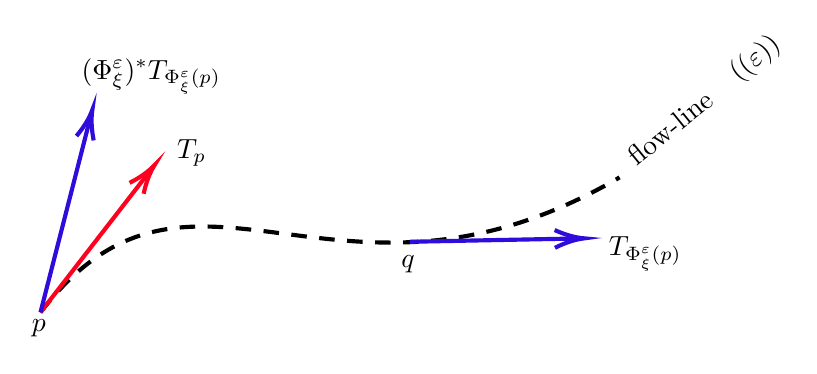
\begin{tikzpicture}[x=0.75pt,y=0.75pt,yscale=-1,xscale=1]
%uncomment if require: \path (0,300); %set diagram left start at 0, and has height of 300

%Curve Lines [id:da8863758369081609] 
\draw [line width=1.5]  [dash pattern={on 5.63pt off 4.5pt}]  (145.68,192.32) .. controls (218.68,97.32) and (287.68,207.32) .. (424.68,127.32) ;
%Straight Lines [id:da25242491594252703] 
\draw [color={rgb, 255:red, 255; green, 0; blue, 31 }  ,draw opacity=1 ][line width=1.5]    (145.68,192.32) -- (198.85,123.69) ;
\draw [shift={(200.68,121.32)}, rotate = 127.76] [color={rgb, 255:red, 255; green, 0; blue, 31 }  ,draw opacity=1 ][line width=1.5]    (14.21,-4.28) .. controls (9.04,-1.82) and (4.3,-0.39) .. (0,0) .. controls (4.3,0.39) and (9.04,1.82) .. (14.21,4.28)   ;
%Straight Lines [id:da3778353955646855] 
\draw [color={rgb, 255:red, 47; green, 11; blue, 220 }  ,draw opacity=1 ][line width=1.5]    (323.68,158.32) -- (404.68,156.73) ;
\draw [shift={(407.68,156.67)}, rotate = 178.87] [color={rgb, 255:red, 47; green, 11; blue, 220 }  ,draw opacity=1 ][line width=1.5]    (14.21,-4.28) .. controls (9.04,-1.82) and (4.3,-0.39) .. (0,0) .. controls (4.3,0.39) and (9.04,1.82) .. (14.21,4.28)   ;
%Straight Lines [id:da5542891074051847] 
\draw [color={rgb, 255:red, 47; green, 11; blue, 220 }  ,draw opacity=1 ][line width=1.5]    (145.68,192.32) -- (169.94,97.57) ;
\draw [shift={(170.68,94.67)}, rotate = 104.36] [color={rgb, 255:red, 47; green, 11; blue, 220 }  ,draw opacity=1 ][line width=1.5]    (14.21,-4.28) .. controls (9.04,-1.82) and (4.3,-0.39) .. (0,0) .. controls (4.3,0.39) and (9.04,1.82) .. (14.21,4.28)   ;

% Text Node
\draw (140,194.4) node [anchor=north west][inner sep=0.75pt]    {$p$};
% Text Node
\draw (318,163.4) node [anchor=north west][inner sep=0.75pt]    {$q$};
% Text Node
\draw (210,107.4) node [anchor=north west][inner sep=0.75pt]    {$T_{p}$};
% Text Node
\draw (418,154.4) node [anchor=north west][inner sep=0.75pt]    {$T_{\boldsymbol{\Phi}^\varepsilon_\xi(p)}$};
% Text Node
\draw (424.99,114.8) node [anchor=north west][inner sep=0.75pt]  [rotate=-321.06] [align=left] {flow-line};
% Text Node
\draw (473.35,73.28) node [anchor=north west][inner sep=0.75pt]  [rotate=-321.1]  {$( \upsigma ( \varepsilon ))$};
% Text Node
\draw (164,68.4) node [anchor=north west][inner sep=0.75pt]    {$\qty(\boldsymbol{\Phi}^\varepsilon_\xi)^* T_{\boldsymbol{\Phi}^\varepsilon_\xi(p)}$};


\end{tikzpicture}

    \caption{Lie transport of a vector along the flow-line generated by some vector field $\boldsymbol{\xi}$}
\end{figure}
\noindent
So for $q$ with coordinates $x'^\mu$, we first need to bring the vector there back to the vector at $p$ (so that these are both in the same vector space) and then compare. This `bringing back' is what is done by the \textit{pullback}.\\[0.2cm] As a final scare I am going to specify the definition of Lie derivative according to the above intuition. Consider $\boldsymbol{\Phi}^\varepsilon_\xi$ to be the map which takes points along a flow-line and consider the vector field $T$, which will take values $T_p$ at point $p$ and $T_q$ at point $q$. Thus $T_p$ and $T_q$ are tangent vectors at those points. Now, $q$ can be written as $\boldsymbol{\Phi}^\varepsilon_\xi(p)$ and thus the tangent vector at $q$ is then $T_{\boldsymbol{\Phi}^\varepsilon_\xi(p)}$.\\[0.2cm] Now let us denote the pull-back map by $\qty(\boldsymbol{\Phi}^\varepsilon_\xi)^*$ which will act on the vector field $T_q$. Note that since $\boldsymbol{\Phi}^\varepsilon_\xi(p)$ generates the flow, we need to define the pullback with respect to this map only. And then the Lie derivative compares between the dragged vector and the original vector,
\begin{align*}
    \SL_{\boldsymbol{\xi}} T(p) = \lim\limits_{\varepsilon\to 0} \frac{\qty(\boldsymbol{\Phi}^\varepsilon_\xi)^* T_{\boldsymbol{\Phi}^\varepsilon_\xi(p)} - T_p}{\varepsilon}
\end{align*}
This is as fas as I can go due to my own inability to understand these complex math stuff. Hence for now, we will shove this into a box and move on with a much simpler definition of Lie derivative using coordinate transformations. 
\subsection{Lie Derivative of a scalar field}
Under a coordinate transformation, we define the \textit{Lie derivative} of a scalar as follows:
\begin{align*}
    \SL_{\boldsymbol{\xi}}\varphi :&= \lim\limits_{\varepsilon\to 0} \frac{\varphi(x')-\varphi'(x')}{\varepsilon}\\
    &=\lim\limits_{\varepsilon\to 0}\frac{1}{\varepsilon}\qty[\varphi(x^\alpha + \varepsilon \xi^\alpha)-\varphi(x^\alpha)]\\
    &=\lim\limits_{\varepsilon\to 0}\frac{1}{\varepsilon}\qty[\varphi(x^\alpha) + \varepsilon\pdv{\varphi}{x^\alpha} \xi^\alpha-\varphi(x^\alpha)]\\
    &=\xi^\alpha \partial_\alpha \varphi
\end{align*}
Since for scalars, covariant and partial derivatives coincide, we can write 
$$\boxed{\SL_{\boldsymbol{\xi}}\varphi = \xi^\alpha \covd{\alpha} \varphi}$$
Hence the Lie derivative of a scalar field under some coordinate transformation generated by $\boldsymbol{\xi}$, is just the `directional derivative' along $\boldsymbol{\xi}$. 
\subsection{Lie Derivative of a contravector field}
In similar lines to the above, we can define the Lie derivative of a contra-vector as
\begin{align*}
    \SL_{\boldsymbol{\xi}} V^\mu :&= \lim\limits_{\varepsilon\to 0} \frac{V^\mu(x')-V^{\mu'}(x')}{\varepsilon}\\
    &=\lim\limits_{\varepsilon\to 0}\frac{1}{\varepsilon}\qty[V^\mu(x^\alpha + \varepsilon \xi^\alpha)-\trmat{\mu}{\beta}V^\beta(x^\alpha)]\\
    &=\lim\limits_{\varepsilon\to 0}\frac{1}{\varepsilon}\qty[V^\mu(x^\alpha) + \varepsilon \pdv{V^\mu}{{x^\alpha}} \xi^\alpha-\qty(\tensor{\delta}{^\mu _\beta} +\varepsilon \pdv{\xi^\mu}{{x^\beta}})V^\beta(x^\alpha)]\\
    &=\xi^\alpha\partial_\alpha V^\mu -V^\alpha \partial_\alpha \xi^\mu 
\end{align*}
Now, the above expression can be written in terms of covariant derivatives.
\begin{align*}
    \SL_{\boldsymbol{\xi}} V^\mu &=\xi^\alpha\qty(\covd{\alpha}V^\mu - \chris{\mu}{\alpha}{\sigma}V^\sigma) -V^\alpha \qty(\covd{\alpha}\xi^\mu -\chris{\mu}{\alpha}{\sigma}\xi^\sigma ) = \qty(\xi^\alpha\covd{\alpha}V^\mu -V^\alpha\covd{\alpha}\xi^\mu)
\end{align*}
The terms with the Christoffel symbols cancel after renaming the dummy indices $\alpha \leftrightarrow \sigma$ in one of the terms. Hence for a contravariant vector we find that 
$$\boxed{\SL_{\boldsymbol{\xi}} V^\mu = \xi^\alpha\covd{\alpha} V^\mu -V^\alpha \covd{\alpha} \xi^\mu}$$ 
\subsection{Lie Derivative of a tensor field}
For our purpose, let us consider a $(0,2)$ tensor field $T$ and consider the change under coordinate transformation.
\begin{align*}
    T'_{\mu\nu}(\fvec{x}') &= \qty(\tensor{\delta}{^\alpha _\mu}-\varepsilon \partial_{\mu}\xi^\alpha)\qty(\tensor{\delta}{^\beta _\nu}-\varepsilon \partial_{\nu}\xi^\beta)T_{\alpha\beta}(\fvec{x})\\
    &=T_{\mu\nu}(\fvec{x}) -\varepsilon\qty(\partial_{\nu}\xi^\beta T_{\mu\beta} + \partial_{\mu}\xi^\alpha T_{\alpha\nu}) + \SO(\varepsilon^2)
\end{align*}
Then let us calculate the difference:
\begin{align*}
   T_{\mu\nu}(\fvec{x}') -T'_{\mu\nu}(\fvec{x}') &=  T_{\mu\nu}(\fvec{x}+\varepsilon \boldsymbol{\xi}) - T_{\mu\nu}(\fvec{x}) +\varepsilon\qty(\partial_{\nu}\xi^\beta T_{\mu\beta} + \partial_{\mu}\xi^\alpha T_{\alpha\nu})\\
   &=\cancel{T_{\mu\nu}(\fvec{x})} +\varepsilon \xi^\rho \partial_\rho T_{\mu\nu}(\fvec{x}) -\cancel{T_{\mu\nu}(\fvec{x})} +\varepsilon\qty(\partial_{\nu}\xi^\beta T_{\mu\beta} + \partial_{\mu}\xi^\alpha T_{\alpha\nu})
\end{align*}
Then from the previous definition the Lie derivative is found out to be:
\begin{align*}
   \boxed{ \SL_{\boldsymbol{\xi}}T_{\mu\nu} =\xi^\rho \covd{\rho} T_{\mu\nu} + \covd{\nu}\xi^\beta T_{\mu\beta} + \covd{\mu}\xi^\alpha T_{\alpha\nu}}
\end{align*}
\subsection{Killing vectors}
We can now characterise the isometries of the metric by defining them to be transformations under which the Lie derivative of the metric vanishes, that is, 
$$\SL_{\boldsymbol{\xi}}g_{\mu\nu} = 0$$
Such a vector field $\boldsymbol{\xi}$ is called a \textit{Killing vector field}. From the expression above of the Lie derivative of a $(0,2)$ tensor field, the above condition becomes,
$$\SL_{\boldsymbol{\xi}}g_{\mu\nu} = \xi^\rho \covd{\rho} g_{\mu\nu} + \covd{\nu}\xi^\beta g_{\mu\beta} + \covd{\mu}\xi^\alpha g_{\alpha\nu}$$
From metric compatibility, we know that $\covd{\rho} g_{\mu\nu} =0$ and hence the first term vanishes. And we can put the metric inside the covariant derivatives in the remaining terms, which will lower the indices of $\xi$. We finally obtain:
$$\SL_{\boldsymbol{\xi}}g_{\mu\nu} \equiv \covd{\mu}\xi_{\nu}+\covd{\nu}\xi_{\mu} =0$$
This is a differential equation, referred to as the \textit{Killing equation}. After solving this, we will get the Killing vector fields which will provide us with the isometries of the metric. \\[0.2cm]
\textbf{FUN FACT}: The collection of all isometries form a group, called the \textit{isometry group} and it is typically a Lie group. The Killing vector fields are the \textit{generators} of this Lie group. \\[0.2cm]
Reflection might also be an \textit{isometry} of the metric, however, these are discrete transformations and hence cannot be obtained from the Killing equation, since these only generate the continuous transformations.